\section{Conditionals}

\subsection{If Else Statements}
\begin{frame}[fragile]{If and Else}{}
    \begin{block}{}
        The \textbf{else} statement is optional.
    \end{block}
    \begin{minted}{c++}
        if (temperature >= 38)
            cout << "Buy an ice ceam cone" << endl;
    \end{minted}
    \pause
    \begin{minted}{c++}
        else
            cout << "Buy a lollipop" << endl;
    \end{minted}
    \pause
    \begin{block}{}
        Must use a block (surrounded by curly braces) for more than one line.
    \end{block}
    \begin{minted}{c++}
        if (number_of_lines > 1) {
            cout << "More than one line.";
            cout << "Have to use a block.";
        }
        else {
            cout << "Curly braces are optional.";
        }
    \end{minted}
\end{frame}

\begin{frame}[fragile]{Cascading}{}
    \begin{center}
        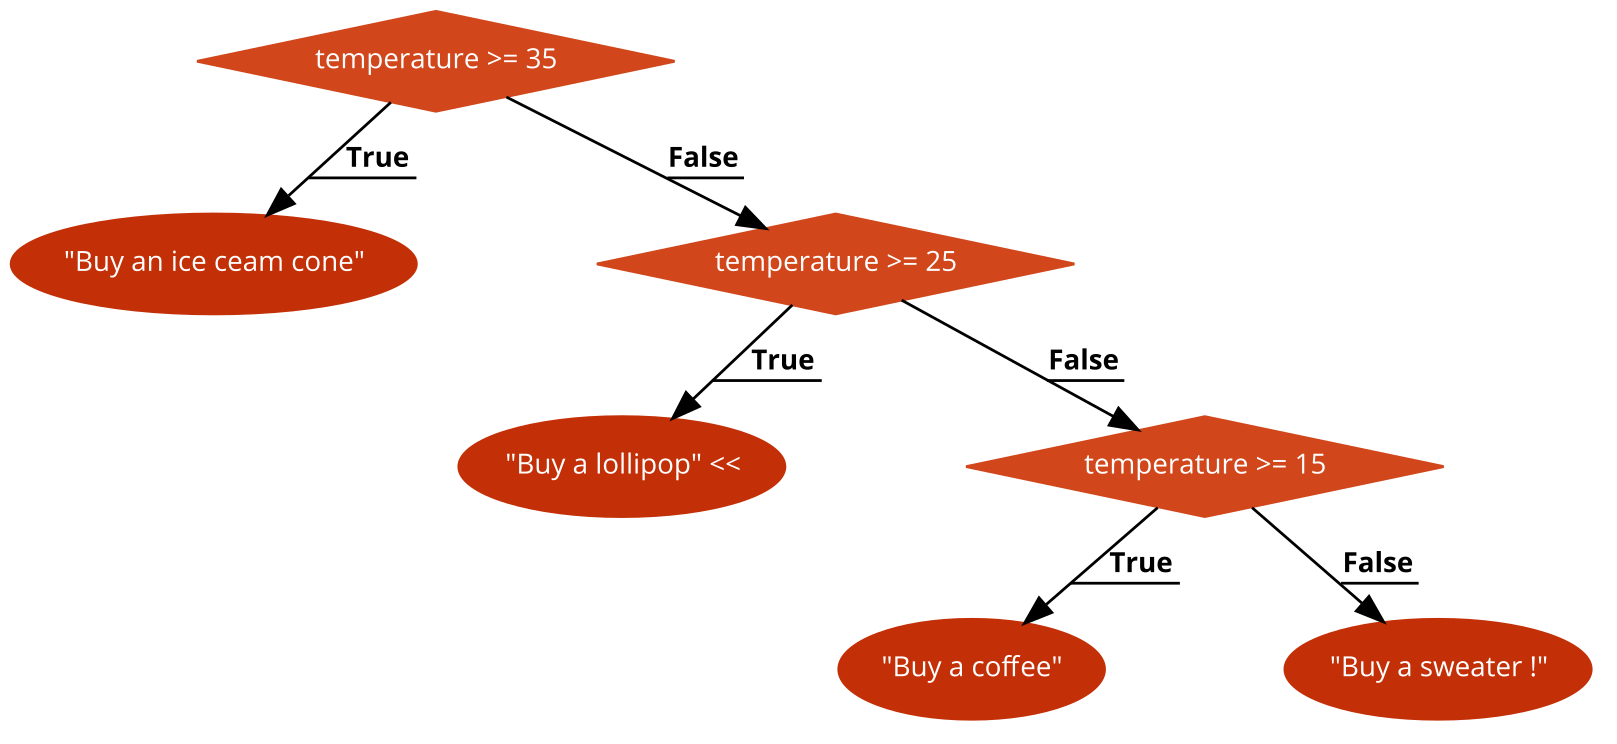
\includegraphics[width=\linewidth]{images/cascading.png}
    \end{center}
\end{frame}

\begin{frame}[fragile]{The \textbf{if...else if...else} Statement}{}
    \begin{block}{}
        To test multiple conditions, we can cascade if statements
    \end{block}
    \begin{minted}{c++}
        if (temperature >= 35) {
            cout << "Buy an ice ceam cone" << endl;
        }
        else if (temperature >= 25) {
            cout << "Buy a lollipop" << endl;
        }
        else if (temperature >= 15) {
            cout << "Buy a coffee" << endl;
        }
        else {
            cout << "Buy a sweater !" << endl;
        }
    \end{minted}
\end{frame}

\begin{frame}[fragile]{The \textbf{if...else if...else} Statement}{}
    \begin{itemize}
        \item The first statement must be an \textbf{if}.
        \pause
        \item After this, there can be any number of \textbf{else if} statements. 
        \pause
        \item At the end, there can be one (or zero) \textbf{else} statement. 
    \end{itemize}
\end{frame}

\subsection{Nested Conditionals}
\begin{frame}[fragile]{Nesting}{}
    \begin{center}
        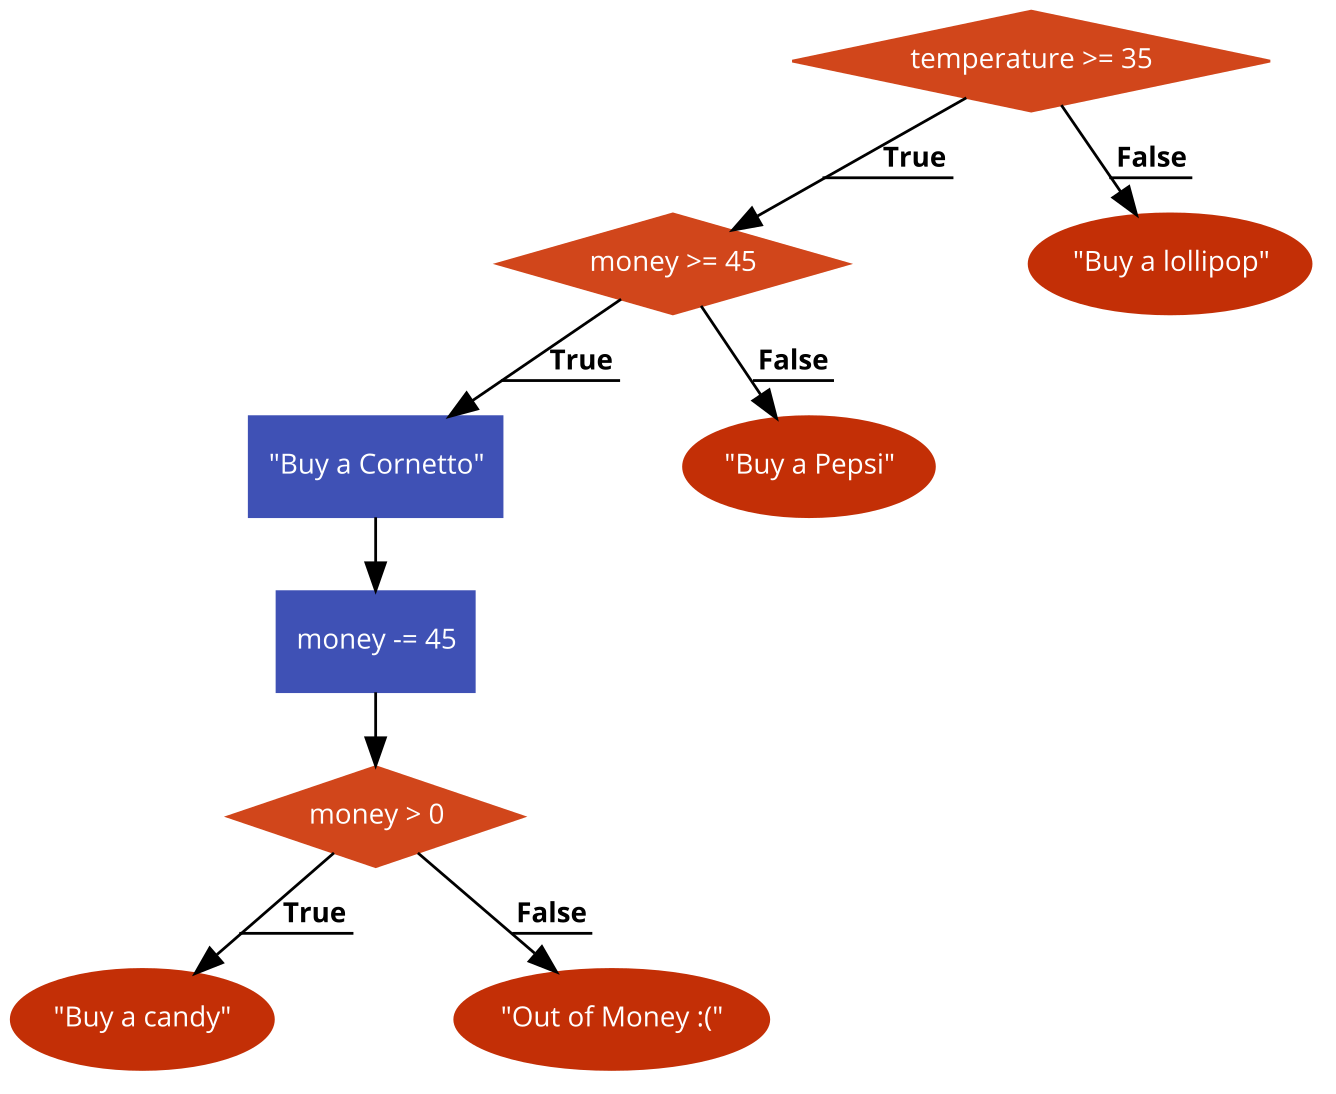
\includegraphics[width=0.7\linewidth]{images/nesting.png}
    \end{center}
\end{frame}

\begin{frame}[fragile]{Nested Conditionals}{}
    \begin{minted}{c++}
        if (temperature >= 35) {
            if (money >= 45) {
                cout << "Buy a Cornetto" << endl;
                money -= 45;
                if (money > 0) {
                    cout << "Buy a candy" << endl;
                }
                else
                    cout << "Out of Money :(" << endl;
            }
            else
                cout << "Buy a Pepsi" << endl;
        }
        else {
            cout << "Buy a lollipop" << endl;
        }
    \end{minted}
\end{frame}

\subsection{Exercises}

\begin{frame}[fragile]{Lab Time !}{Write programs for each of the following specifications}
    \begin{block}{~\vspace{0.5cm}}
    \begin{center}
    \vspace{-0.6cm}
    \begin{tabular}{p{0.45\textwidth}|p{0.45\textwidth}}
        \textcolor{white}{\bf Input} & \textcolor{white}{\bf Output} \\
        Four integers &
        Maximum and second max value \\ \hline
        Cutoff for A, B, C grades, and also marks of one student (out of 100) &
        1. Are the cutoffs valid ?\hfill\hspace{3em} 2. Student's grade (A,B,C) \\ \hline
        Three points (vertices of triangle) in terms of $(x,y)$ coordinates &
        Whether the triangle is equilateral, isosceles, or scalene
    \end{tabular}
    \end{center}
    \end{block}
    \begin{block}{}
        Write a program that takes as input, the coefficients of a quadratic equation
        ($Ax^2+Bx+C$), and outputs the roots (both real and imaginary).
    \end{block}
    \setbeamercolor{block title}{use=structure,fg=white,bg=red!35!black}
    \begin{block}{Sorting}
        Write a program that accepts $N$ numbers as input,
        and prints them out in ascending order.
    \end{block}
\end{frame}

